% Journal of Computational Sciences
\documentclass[3p]{elsarticle}

% PACKAGES
\usepackage{graphicx, amsmath, amssymb, amsfonts, mathtools, mathrsfs, color}
\usepackage{comment, enumerate, tabularx, multirow}
\usepackage{natbib, hyperref, url}
\usepackage{algorithm, algpseudocode, pifont, longtable}
%\usepackage[justification=RaggedRight]{caption}


%^^^^^^^^^^^^^^^^^^^^^^^^^^^^^^^^^^^^^^^^^^^^^^^^^^^^^^^^^^^^%
% COMMANDS
% Basic editing
\newcommand{\tocite}{{\color{blue}(to cite)}}
\newcommand{\vsp}[1]{\vspace{#1 pc} \noindent}
\newcommand{\np}{\newpage \noindent}
\newcommand{\HERE}[1]{ \vsp{#1} {\color{blue} HERE} }
\newcommand{\tofix}{\color{blue}}
\newcommand{\new}{}		% \color{green}
\newcommand{\newa}{}		% \color{red}
\newcommand{\newb}{}		% \color{blue}
% Basic math, derivatives
\newcommand{\td}[2]{\frac{d #1 }{d #2}}
\newcommand{\ttd}[2]{\frac{d^2 #1 }{{d #2}^2}}
\newcommand{\pd}[2]{ \frac{ \partial #1}{ \partial #2 } }
\newcommand{\ppd}[2]{ \frac{ \partial^2 #1}{ {\partial #2}^2 } }
% Basic math, vectors and other
\newcommand{\BigO}[1]{ \mathcal{O} \left(#1\right) }
\newcommand{\bvec}[1]{\ensuremath{\boldsymbol{#1}}}
\newcommand{\grad}{\nabla} 
\newcommand{\abs}[1]{\left| #1 \right|}
\newcommand{\tavg}[1]{\langle #1 \rangle}
\newcommand{\norm}[1]{ \left\| #1 \right\| }
\newcommand{\ip}[1]{ \langle #1 \rangle }
% For real and imaginary, could use \Re or \Im, or \mathcal{R}, or \text{Re}
%^^^^^^^^^^^^^^^^^^^^^^^^^^^^^^^^^^^^^^^^^^^^^^^^^^^^^^^^^^^^%


%^^^^^^^^^^^^^^^^^^^^^^^^^^^^^^^^^^^^^^^^^^^^^^^^^^^^^^^^^^^^%
% TITLE AUTHORS ABSTRACT
\begin{document}
%\title{An eroding porous medium}
\title{The development of anisotropy in an eroding porous medium}
%
\author[Nick]{M.~Nicholas J.~Moore}
\author[Bryan]{Bryan D.~Quaife}
\address[Nick]{Department of Mathematics and Geophysical Fluid Dynamics Institute, Florida State University, Tallahassee, FL, 32306.}
\address[Bryan]{Department of Scientific Computing and Geophysical Fluid Dynamics Institute, Florida State University, Tallahassee, FL, 32306.}
\begin{abstract}
We numerically simulate the erosion of a porous medium due to an internally flowing fluid. The solid constituents of the porous medium erode under the action of surface shear stress. As the particles shrink, they elongate in the direction of the flow, giving rise to anisotropic conductivity of the porous medium.
\end{abstract}
\maketitle
%^^^^^^^^^^^^^^^^^^^^^^^^^^^^^^^^^^^^^^^^^^^^^^^^^^^^^^^^^^^^%

\newpage
\section{Introduction}
Stuff \cite{Ristroph2012, Moore2013, Huang2015, MooreCPAM2017} and other stuff \cite{Rycroft2016, Mitchell2016}.


%^^^^^^^^^^^^^^^^^^^^^^^^^^^^^^%
\begin{figure}%[htbp]
\begin{center}
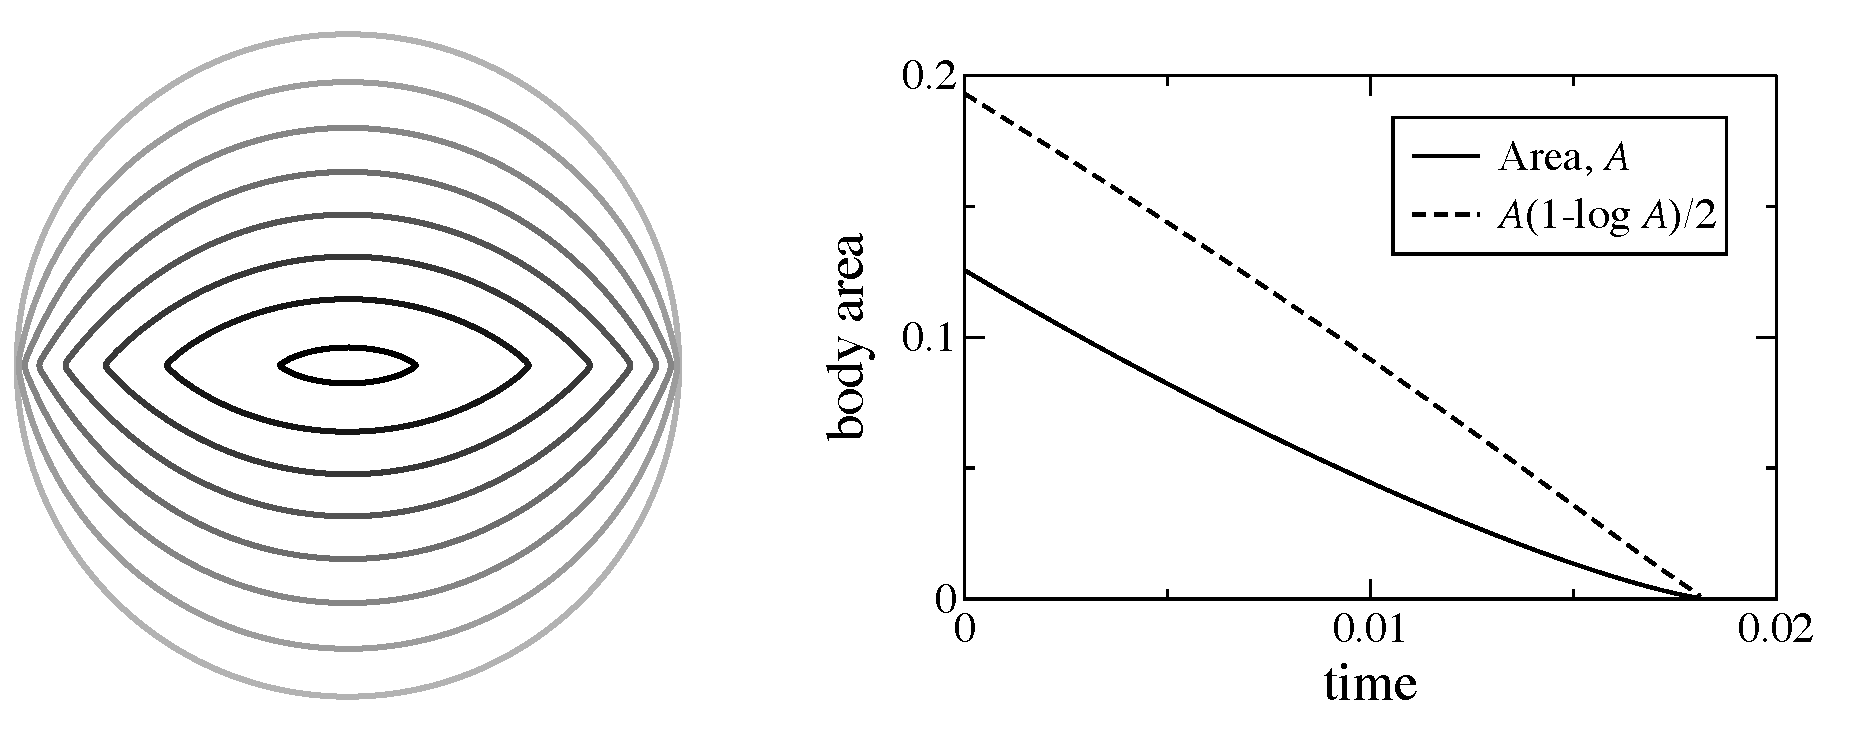
\includegraphics[width = 0.9 \textwidth]{./Figs/fig1.pdf}
\caption{Shrinking body and area.}
\label{fig1}
\end{center}
\end{figure}
 %^^^^^^^^^^^^^^^^^^^^^^^^^^^^^^%

%^^^^^^^^^^^^^^^^^^^^^^^^^^^^^^%
\begin{figure}%[htbp]
\begin{center}
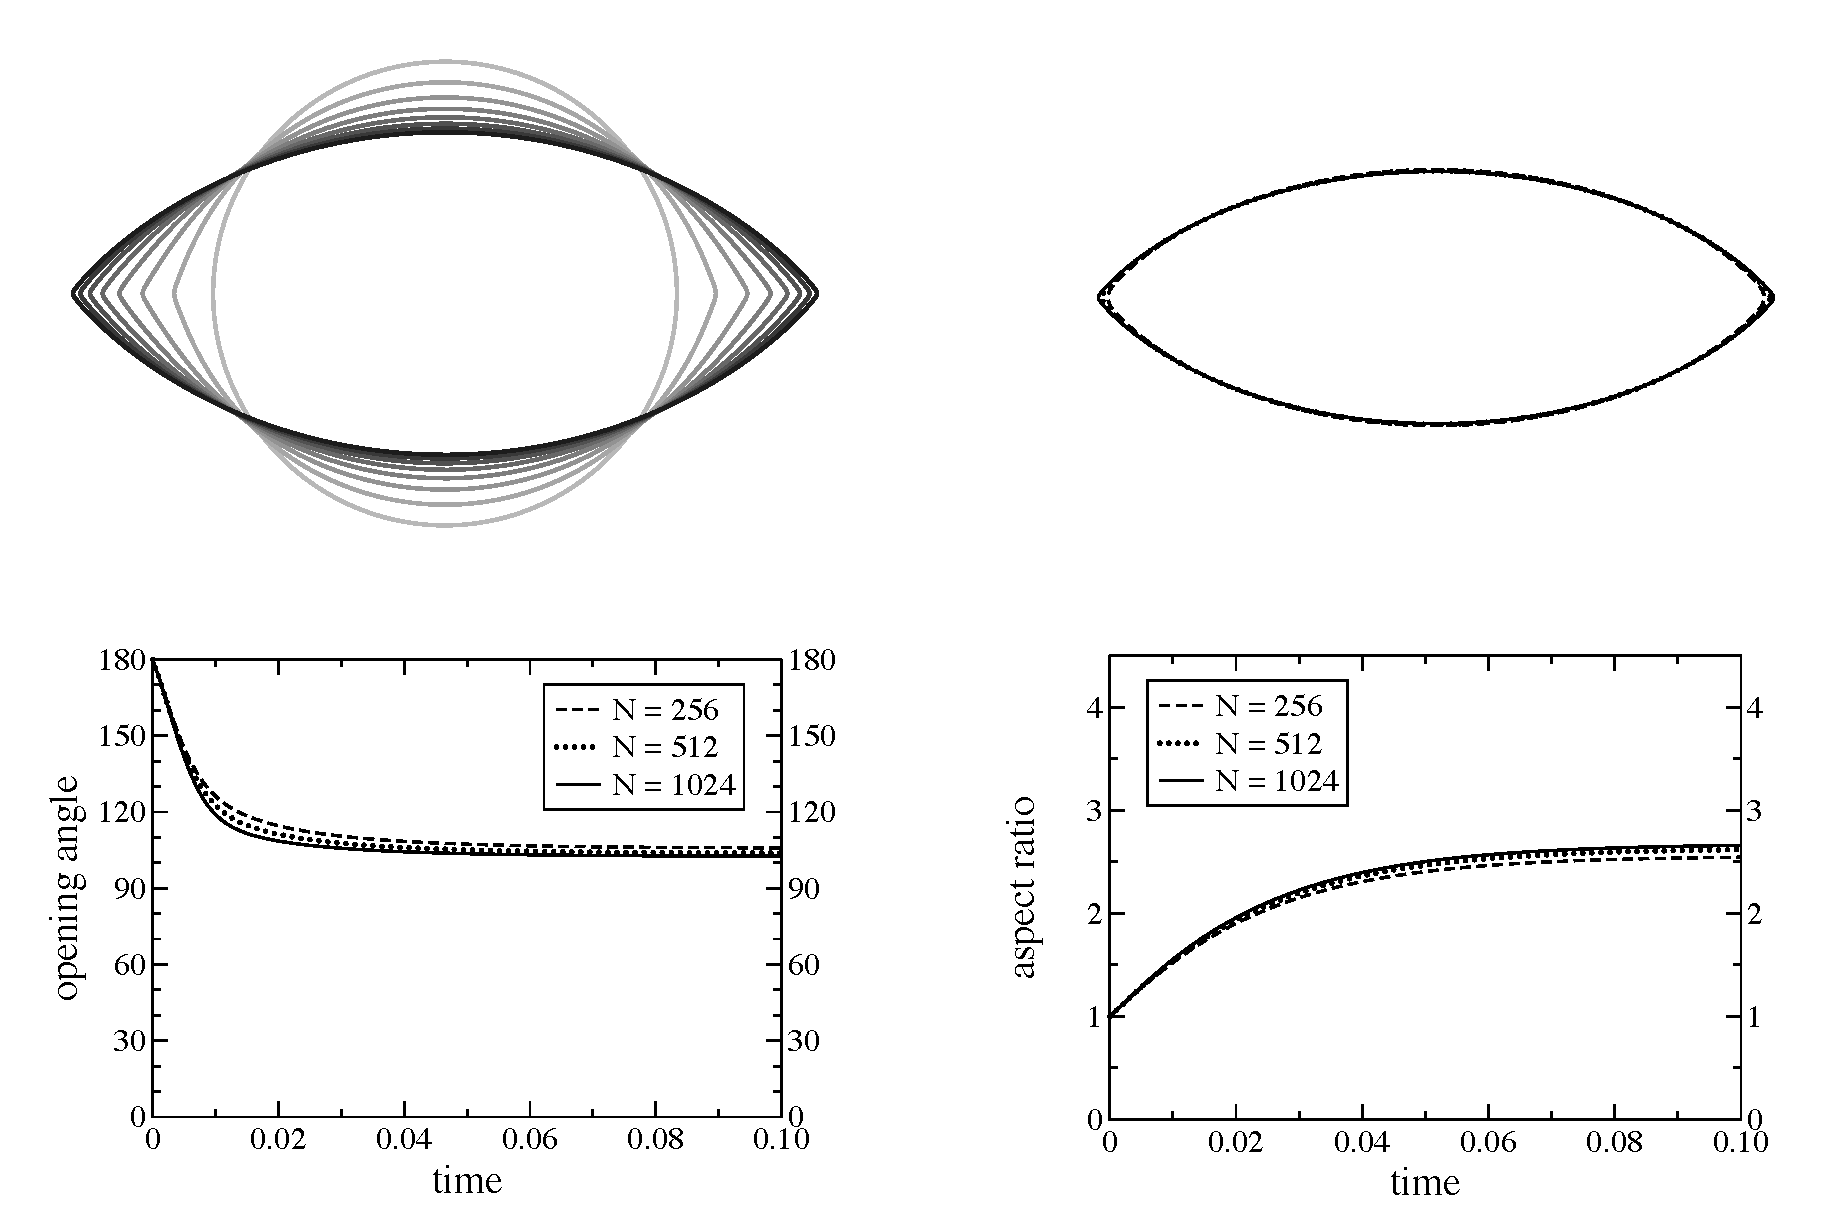
\includegraphics[width = 0.99 \textwidth]{./Figs/fig2.pdf}
\caption{Final shape.}
\label{fig2}
\end{center}
\end{figure}
 %^^^^^^^^^^^^^^^^^^^^^^^^^^^^^^%

\bibliographystyle{plain}
\bibliography{refs}
\end{document}
